\documentclass{article}
\usepackage[utf8]{inputenc}
\usepackage[backend=biber,
style=numeric,
citestyle=numeric]{biblatex}
\usepackage{url}
\usepackage{csquotes}
\usepackage{pgfplots}
\usepackage{pgfplotstable}
\pgfplotsset{compat=1.7}
\usepackage{tikz}
\usepackage{hyperref}
\usepackage{graphicx}
\usepackage{amssymb}
\usepackage{amsmath}

\addbibresource{citations.bib}
\graphicspath{{images/}}

\title{Detecting Spurious Correlations in Image Annotations}
\author{Felix Möller}
\date{August 10th, 2021}

%TODO-Meta: Autorennamen raus,
\begin{document}
\maketitle
\tableofcontents
\newpage
\section{Abstract}
%TODO: Abstract besser formulieren (interpretability raus, kein "ich")
Neural networks and especially Convolutional Neural Networks (CNN) have revolutionized the field of computer vision in the recent years.
While neural networks become more refined every year they also become more complex and difficult to interpret.
However, interpretability is important because it allows researchers to investigate whether their models make
their predictions by "learning from the right thing" or not. Surprisingly, recent research has shown that many models' predictions
rely on so-called spurious correlations. In this report, I will present an overview over the existing methods
to detect spurious correlations and compare them with regard to their usability.
Next, I will show what should and what should not be done to mitigate the impact of spurious correlations on classification
accuracy and finally I will propose a workflow to handle datasets that could contain spurious correlations. 


\section{Introduction}
\subsection{What is a spurious correlation (s.c.)?}
%TODO: 2.1 ersten Satz weglassen, co-movement raus, welche s.c.s nicht
Before we have a look at the impact of spurious correlations on image datasets we first need to focus on what spurious correlations are.
According to \cite{sc_def} a spurious correlation is a \enquote{connection between to variables that appears causal but is not}.
This means that there \textit{appears} to be a logical explanation for the co-movement of both variables when the correlation is in fact completely random.
\hyperref[sec:challenges]{Section 2.4} mentions why this is especially problematic in a machine learning context.
In this report, I will only have a look at spurious correlations that exist between a given feature of the dataset (e.g. the background of the image)
and the target value (e.g. the age of a person) as these are the only spurious correlations that might cause the classifier to make wrong generalizations.


\subsection{Common types of s.c.s in image datasets}
Modern research has worked out two commonly occurring types of spurious correlations. The first one is between \textbf{image angle} and \textbf{target} \cite{5995347}.
In datasets that contain such a spurious correlation, the target is often shown from a similar angle (e.g. in an image dataset made up of cars all cars
could be shown from the front) or in the same part of the image (e.g. most of the time the object of interest is in the centre of the image).
Spurious correlations between image angle and target can be problematic because an image recognition model trained on a dataset
which contains such a spurious correlation might struggle to classify the target object when it is shown from an angle that was not present in the training dataset. \\
The next commonly occurring spurious correlation between \textbf{context} and \textbf{target} \cite{Singh_2020_CVPR}.
Spurious correlations between context and target occur in datasets where a non-target object co-occurs with the target object.
One example would be cars which are commonly depicted with people. A classifier trained on a dataset with a spurious
correlation between context and target might infer that the target value has to occur with its spuriously correlated non-target
object. So in our car example, a classifier might only detect a car if a person is also present in the image.


\subsection{Why study spurious correlations?}
\label{sec:motivation}
Datasets containing spurious correlations can significantly diminish the accuracy of a model compared to training on a dataset
where no spurious correlations are present. Kim et al. have shown how much varying degrees of the same spurious correlation
impact the classification accuracy of a model \cite{Kim_2019_CVPR}. They planted a spurious correlation between a digit and its
color into the classic MNIST dataset \cite{mnist_web}, meaning they assigned a mean color to every digit in the training set and
then drew from $N(mu_{digit},{\sigma^2}_{train})$ where $mu_{digit}$ is the mean color of the given digit and
${\sigma^2}_{train}$ is the variance of the normal distribution which was altered between iterations.
The digits in the test dataset were assigned a random color (i.e. the mean color was not digit-specific), indicating that there
is no spurious correlation in the test dataset. The degree of the spurious correlation between digit and color in the training
set depends on ${\sigma^2}_{train}$ with a low value indicating a high degree of the spurious correlation and vice-versa.
The evaluation results can be seen in  \hyperref[fig:mnistGraph]{Figure 1}. Although the spurious correlation would most likely
be noticed in practice for very low $\sigma^2$, it is clear to see that even for the highest $\sigma^2$ the drop in
classification accuracy is still significant (keep in mind that state-of-the-art classifiers can easily obtain above
95 \% test accuracy on the MNIST dataset \cite{mnist_web}).

\begin{figure}
    \centering
    \begin{tikzpicture}[scale=0.8]
    \begin{axis}[
        xlabel = $\sigma^2$,
        ylabel = Accuracy,
        width=10cm,
        height=7cm,
    ]
    \addplot[color=red, mark=.] coordinates {
        (0.02,0.4)
        (0.025,0.48)
        (0.03,0.6)
        (0.035,0.66)
        (0.04,0.73)
        (0.045,0.8)
        (0.05, 0.84)
    };
    \end{axis}
    \end{tikzpicture}
    \caption{Effect of a spurious correlation between color and digit on classification accuracy
    in the classic MNIST dataset. A lower variance indicates a more severe spurious correlation and vice-versa.}
    \label{fig:mnistGraph}
\end{figure}


\subsection{Why is detecting s.c.s in image datasets difficult?}
\label{sec:challenges}
Detecting spurious correlations in a given dataset is a challenge, regardless of whether the dataset contains
text data, plain numbers or images. The problem remains to evaluate if a given correlation is spurious or not.
Whilst determining the causality of a correlation is often easy for humans because they are able to make use of
their human intuition, computers would have to inspect an infinite amount of images to classify a correlation as
(not) spurious. However a machine-learning model only has a limited amount of data to train on and the training
set it is given could misrepresent the concept it is trained for (i.e. contain spurious correlations). \\
In such a case, the model would most likely rely on the spurious correlation(s) which is present in the training set.
An additional challenge in the context of image datasets is feature-extraction. Determining the correlation
between a given feature of a dataset and the target attribute (e.g. the correlation between the presence of a special word
and target attribute) can be automated when the feature is annotated. Extracting high-level features such as
the location of an object in an image or the image angle it is captured from would require training
an additional classifier to detect the concept. Such a classifier could however make its predictions by exploiting spurious
correlations which makes this way of feature-extraction unreliable. \\
The last option is to inspect the dataset manually. While this is the most reliable method to detect spurious correlations,
the sheer size of modern image datasets (IMDB-WIKI: 523,000 images \cite{Rothe-ICCVW-2015}, MS COC0: 328,000 images 
\cite{lin2015microsoft}) makes manual detection of spurious correlations infeasible.


\section{Detecting spurious correlations}
%TODO: die ersten beiden Sätze raus
Despite the significant negative impact of spurious correlations on classification accuracy,
detecting spurious correlations remains largely unexplored to this day.
Nevertheless researchers have proposed a handful of algorithms to detect spurious correlations
in image datasets. These can be grouped into two categories: The first one is \textbf{human-based detection}
which relies on inspecting a dataset manually to detect spurious correlations. Although I have mentioned that
manually inspecting image datasets is not feasible in \hyperref[sec:challenges]{Section 2.4},
there are algorithms which rely on humans to detect spurious correlations. One member of this category is
Crowdsourcing \cite{10.1145/3366423.3380063}, which makes use of volunteers to speed up the detection process and increase its reliability. \\
The second category is \textbf{Detection via model explanations}. Methods belonging to this category inspect a model trained on
the given dataset to check if the model exploits spurious correlations to make its predictions.
This can either be done by highlighting the parts of an image which contributed to the classification or by testing if the
model responds to a user-defined concept. Gradient-weighted Class Activation Mapping (Grad-CAM) \cite{Selvaraju_2017_ICCV}
makes use of the former, while Testing with concept activation vectors (TCAV) \cite{pmlr-v80-kim18d} relies on the latter.

\subsection{Crowdsourcing}
The main principle of Hu et al.'s Crowdsourcing approach \cite{10.1145/3366423.3380063} is to distribute the given dataset
among all multiple volunteers to reduce the individual effort of each person. A brief summary of their approach
can be seen in \hyperref[fig:crowdsourcing]{Figure 2}. \\
Their proposed algorithm consists of three steps: \textbf{Step 1} is called \textbf{Question generation}.
In this step each volunteer is provided with a random sample of the dataset. Next, each volunteer creates questions regarding
anomalies he has found in his sample of the dataset where the answer to such a question is the given anomaly
(the answer is also given by the volunteer). Between step 2 and step 1 all similar questions are merged via spaCy,
an open-source natural language processing tool \cite{spaCy}. \\
In \textbf{Step 2} which is called \textbf{Answer collection} the dataset is again randomly distributed among the volunteers
of this step. Note that a volunteer only participates in one step of the process to increase its reliability.
Among with a sample of the dataset a volunteer is confronted with question generated in step 1 which he answers with the
anomaly he sees in his sample of the dataset. If the volunteer sees no anomaly in his sample, he can skip the question.
Between steps 2 and 3 a weight $w_{i,2}$ is assigned to each potential spurious correlation $i$ which is the fraction of
volunteers who provided the most common answer (similar answers to a question are merged).
In addition, each question is transformed into a statement. \\
In \textbf{Step 3} which is called \textbf{Bias Judgement} another group of volunteers is confronted with the statements
generated at the end of step 2. Most importantly, the volunteers do not see the dataset.
They then have to answer whether or not the given statements reflect the real world (yes/no answers only).
At the end of step 3 another weight $w_{i,3}$ is assigned to each potential spurious correlation $i$ which is the fraction
of workers stating that the statement belonging to a potential spurious correlation is not an accurate
reflection of the real world. \\
After step 3, the total weight $W_{i}=w_{i,2} \cdot w_{i,3}$ is assigned to each potential spurious correlation the idea
behind the computation of the total weight is that the severity of each potential spurious correlation is determined by
how abnormal it is (determined in step 3)\textit{and} by how present it is in the dataset (determined in step 2).
All spurious correlations with $W_i > t$ are the output of the algorithm where $t$ is a threshold which can be chosen
by the conductors of the algorithm. \\

\begin{figure}
    \centering
    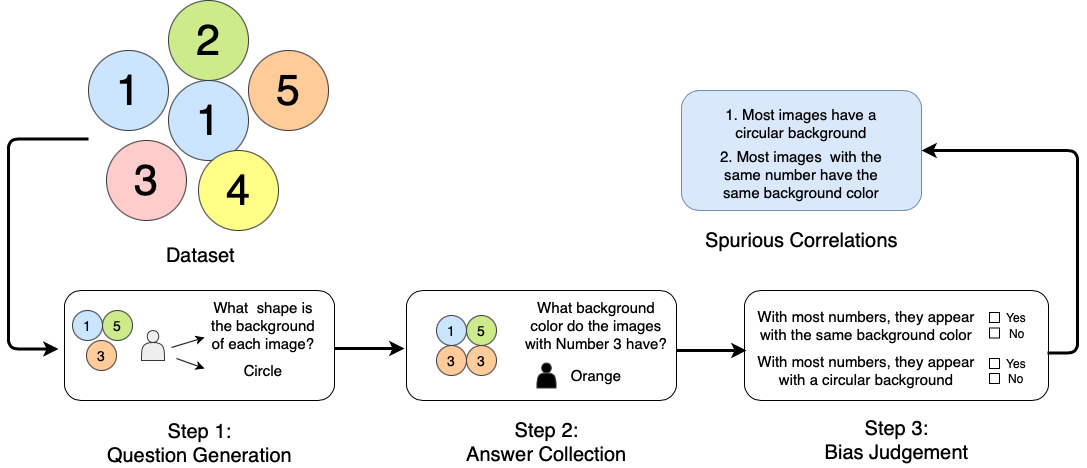
\includegraphics[scale=0.315]{crowdsourcing.png}
    \caption{Crowdsourcing approach to detect spurious correlations in image datasets, proposed by Hu et al. \cite{10.1145/3366423.3380063}}
    \label{fig:crowdsourcing}
\end{figure}

Overall, Crowdsourcing can be seen as an effective algorithm because it largely relies on human intuition to detect
spurious correlations. An additional benefit of this approach is that it is conducted by working directly
on the dataset which makes it superior to model explanations. \\
In both studies conducted by Hu et al. more than 10 volunteers per 100 images took part in the study.
Even if one were to inspect only a small fraction of the dataset, one would need in excess of 100 volunteers!
The fact that Crowdsourcing relies on such a large amount of volunteers is ambivalent. On the one hand, relying on multiple
volunteers decreases the bias towards the perceptions of a small group and leads to finding more spurious correlations.
However to most people needing to inspect a dataset such a large group of volunteers is unattainable and relying on humans
to detect spurious correlations is time-consuming.
Another problem with Crowdsourcing is that the output often contains incorrect detections.
In the second study conducted by Hu et al. in which the volunteers inspected a car dataset two of the top 10 outputs
were \enquote{No cars have rust} and \enquote{Each car is fueled by gasoline}. \\
In conclusion, Crowdsourcing is an effective approach to detect spurious correlations in image annotations
but the high amount of time and effort it requires make it only applicable to frequently used datasets. 
Automating all three steps would make this approach a lot more efficient. While steps 1 and 2 cannot be automated because the
questions generated and answered have no pattern to them, step 3 could be partially automated by using answers to previous
statements if the statements are similar.


\subsection{Grad-CAM}
%TODO: Zitat Grad-CAM
Grad-CAM highlights the parts of an image that contributed to a given classification by inspecting its
final convolutional layer. An overview of Grad-CAM can be seen in \hyperref[fig:gradcam]{Figure 3}. \\
To generate an explanation for a given image with Grad-CAM, the image is first given to a CNN as its input
and a class $c$ whose contribution should be explained needs to be specified. Grad-CAM then assigns a weight
${w_k}^c$ to each of the $n$ feature maps of the final convolutional layer of the given CNN with
\begin{align*}
    {w_k}^c = \frac{1}{I \cdot J} \sum\limits_{i=1}^{I} \sum\limits_{j=1}^J \frac{\partial y^c}{\partial {A^k}_{i,j}}.
\end{align*}
This can be interpreted as the average importance of each entry of feature map $k$ to the classification of class $c$.
The output of Grad-CAM is computed by adding up all $n$ feature maps multiplied by their respective weight and plugging
them into a ReLU-function. Said differently, the output of Image $i$ with $c$ being the class of interest looks as follows:
\begin{align*}
    O_{Grad-CAM, i, c} = ReLU(\sum\limits_{k=1}^N {w_k}^c \cdot A^k).
\end{align*}
ReLU is applied to filter out parts of the image that
negatively contributed to the classification. Note that the output of Grad-CAM is of the same dimension as each
feature map of the final convolutional layer which is usually much smaller than the dimension of the input image. \\
One advantage of Grad-CAM over other existing explanation algorithms is that its output is class-discriminative,
i.e. it only highlights those parts of the image that positively contributed to the specified class of interest.
However since the output of Grad-CAM is of a smaller dimension than the input image its resolution is often not good enough
to deliver a precise explanation. To combat this, Selvaraju et al. proposed a second approach named Guided Grad-CAM,
which pointwise multiplies the output of a second explanation algorithm named Guided Backpropagation \cite{springenberg2015striving}
with the output of Grad-CAM which is first upscaled to the dimension of the input image. 
Guided Grad-CAM combines the benefits of Grad-CAM whose output is low resolution but class-discriminative and
Guided Backpropagation which delivers an explanation in high resolution without being class-discriminative.
This enables the visualization of fine-grained concepts which the CNN responds to like
the stripes of the tiger-cat in \hyperref[fig:gradcam]{Figure 3}. \\
In conclusion, Grad-CAM is a visual explanation algorithm which can be used to detect spurious correlations
in image datasets by inspecting the predictions of a CNN trained on the dataset of interest and checking whether the regions
highlighted by Grad-CAM fit to concepts that spuriously correlate with the target class.
For example a spurious correlation between gender and profession can be detected by checking whether Grad-CAM
highlights the face of the depicted person or the clothing. 
A huge advantage of Grad-CAM is that it can be applied to any CNN which is currently the state-of-the-art model
for most computer vision tasks. In addition, applying Grad-CAM requires no retraining which saves time in the process
of detecting spurious correlations. Another benefit of Grad-CAM is the simplicity of its output:
Since Grad-CAM explains the classification via a  simple heatmap, the explanation can be understood by anyone
and no machine-learning expertise is needed. 
However, since Grad-Cam explains the classification of a model trained on the dataset of interest,
it can only show the spurious correlations that the given model exploits. This can lead to problems because
different models can rely on different (spurious) correlations when making their predictions.
Another problem of Grad-CAM is that one needs to inspect multiple explanations to confirm that the model
relies on a certain concept when making its predictions. Since this needs to be done manually, it takes up
most time in the detection process and slows it down considerably. Estimating the degree of a spurious correlation
with Grad-CAM is also a challenge because Grad-CAM does not compute a value for a given spurious correlation.
%TODO: DRINGEND Überarbeiten!!!
Research conducted by Tong \& Kagal \cite{tong2020investigating} has shown that most simple metrics fail
to estimate the degree of a spurious correlation when using Grad-CAM because its output is noisy, i.e. it always
highlights features which do not causally correlate with the target even if the dataset does not contain spurious
correlations, only to a lesser extent.

\begin{figure}
    \centering
    \includegraphics[scale=0.057]{grad_cam_overview.png}
    \caption{Overview of Grad-CAM, proposed by Selvaraju et al. \cite{Selvaraju_2017_ICCV}. Grad-CAM explains
    a CNN-model by inspecting its final convolutional layer. The output of Grad-CAM can be pointwise multiplied
    with the output of an algorithm called Guided Backpropagation \cite{springenberg2015striving} to receive a
    more detailed explanation}
    \label{fig:gradcam}
\end{figure}


\subsection{TCAV}
%TODO: Absätze, Ghorbani-Approach, feature extraction 
TCAV \cite{pmlr-v80-kim18d} is an algorithm which detects spurious correlations by testing if a neural network trained
on the dataset of interest relies on a user-defined concept when making its predictions. An overview of the algorithm
can be seen in \hyperref[fig:tcav]{Figure 4} \\
\textbf{Step 1} requires the user to \textbf{define a concept} of interest $c$ (e.g. the stripes of a zebra
or the face of a person). The user then collects a set of images that depict the concept and another set
containing random images that do \textit{not} belong to the concept. Next, the user chooses a layer $l$ from
the neural network which he wants to investigate. \\
In \textbf{Step 2} the images collected in Step 1 are fed into the neural network and a linear classifier is trained
to separate the activations at layer $l$ that belong to the concept from the activations of the random images.
The vector orthogonal to the decision boundary is the \textbf{concept activation vector} $v_c$ for the given concept $c$.\\
In \textbf{Step 3} a \textbf{TCAV-Score} is assigned to the user-defined concept. To do so, a score $S_{c,k}(i)$
is assigned to each image containing class $k$ in the original dataset with 
\begin{align*}
    S_{c,k}(i) = \frac{\partial p_k(i)}{\partial v_c},
\end{align*}
meaning that $S_{c,k}(i)$ is the directional derivative of the prediction probability for class $k$ being present
in image $i$ with regard to the concept activation vector. A positive $S_{c,k}(i)$ implies that the presence of
concept $c$ in image $i$ positively contributed to is classification as class $k$.
The final TCAV-Score for a concept is 
\begin{align*}
    \frac{|i \in I_k: S_{c,k}(i) > 0 |}{|I_k|}
\end{align*}
where $I_k$ is the set of images
in the dataset that contain class $k$. A concept with a high TCAV-Score is most likely a concept that the classifier
relies on when making its predictions. \\
A huge benefit of TCAV is its flexibility towards model architecture: TCAV can be applied to any neural network and
it is even possible to choose the layer which one wants to investigate. In addition, the algorithm can be automated so
that all the user has to do is define the concept. This is important because it allows people without any machine-learning
knowledge to investigate the model. However like Grad-CAM, TCAV is an algorithm that explains a given model an can
therefore only detect spurious correlations which the given model exploits. An even bigger problem is that TCAV can only
check if the model exploits a spurious correlation if the user has the assumption that this is the case.
This means that spurious correlations which do not often occur and are therefore not assumed to be present
in the dataset cannot be detected when detecting spurious correlations solely with TCAV. Another problem with TCAV
is that it suffers from the \enquote{garbage in, garbage out}-principle: a poorly-defined concept can lead to a low
TCAV-Score even if the concept is important. This can happen quite often because properly defining a concept can take time
since one has to carefully select images that adequately represent the concept. Tong \& Kagal therefore propose to choose
images that contain multiple concepts of interest to make the process of concept definition
more efficient \cite{tong2020investigating}.

\begin{figure}
    \centering
    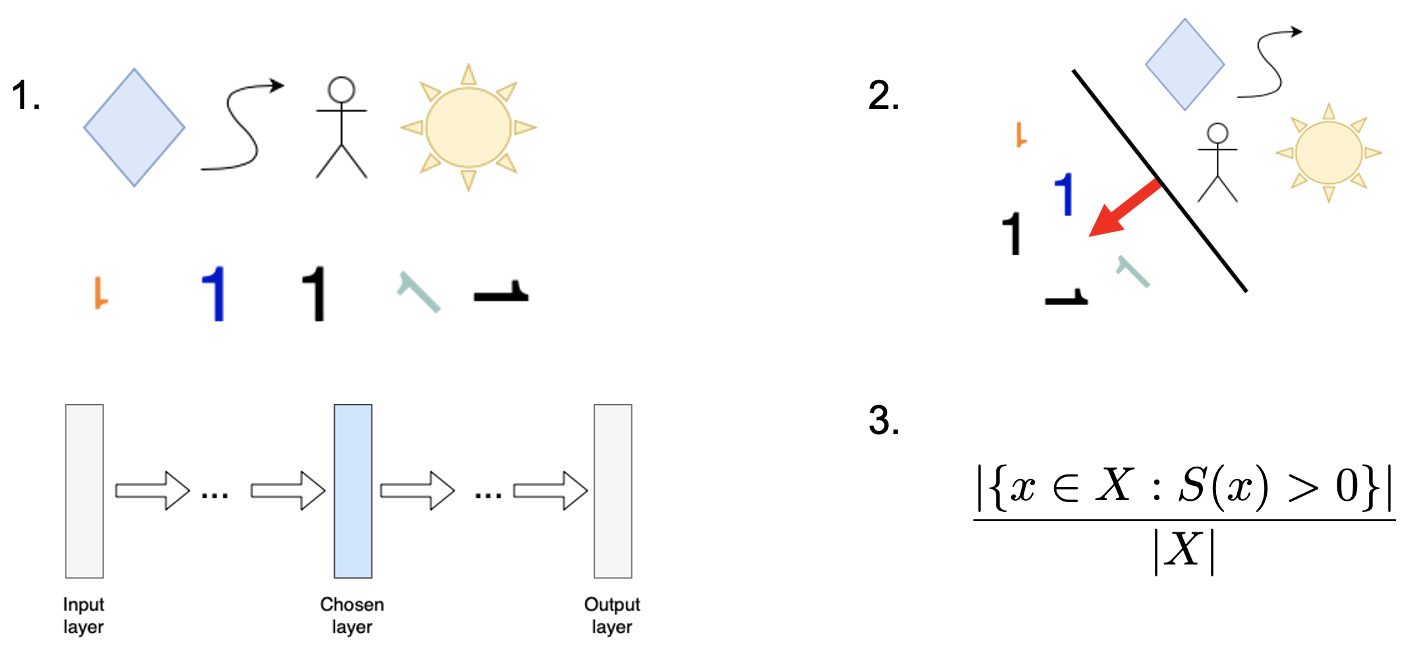
\includegraphics[scale=0.45]{tcav.png}
    \caption{Overview of TCAV, proposed by Kim et al. \cite{pmlr-v80-kim18d}. TCAV can be used to determine if a user-defined
    concept is important for the classification of a neural network. The approach consists of three steps: first,
    the concept of interest is defined and a layer from the neural network is chosen. Next, the concept activation
    vector is computed (marked in red). In the final step, a TCAV-Score is asserted to the concept}
    \label{fig:tcav}
\end{figure}


\subsection{Comparing existing methods to detect spurious correlations}
The three methods to detect spurious correlations mentioned in this report all have different strengths and weaknesses.
However to determine the best method to detect spurious correlations it is beneficial to evaluate the quality of each method
via the same criteria. Tong \& Kagal \cite{tong2020investigating} have proposed 5 criteria which a reliable method to
detect spurious correlations should fulfill. An overview can be seen in \hyperref[tab:comparison]{Table 1}.\\
The first criterion is \textbf{detecting the spurious correlation}. This means that the method itself should detect
the spurious correlation without any input other than the dataset. Grad-CAM and Crowdsourcing fulfill this criterion
but TCAV can only confirm or deny the assumption that a given spurious correlation exists in a dataset. \\
Next, a method to detect spurious correlations should \textbf{detect the degree of the spurious correlation}.
Quantifying different spurious correlations is important to determine how prevalent a spurious correlation is in a dataset.
The experiment shown in \hyperref[sec:motivation]{Section 2.3} demonstrates how differently varying degrees of the same
spurious correlation impact the accuracy of a classifier. Grad-CAM fails to assign a value to each spurious correlation
which makes is challenging to estimate the degree of a spurious correlation. The TCAV-Score and weights assigned by
Crowdsourcing do not allow for a perfect comparison of different spurious correlations because their computation includes
human subjectivity but they at least allow for a rough grouping. \\
The third criterion is \textbf{efficiency} which a detection method fulfills if it requires little time and human effort.
This is the only criterion which no method fulfills because every method requires some form of human effort. Grad-CAM requires
the user to inspect classifications, with TCAV the user needs to collect images for a concept and Crowdsourcing involves
human effort in every step. Although all methods require human effort Crowdsourcing stands out among TCAV and Grad-CAM
not only because of the amount of human effort it requires but especially for the fact that a high number of
volunteers is needed. \\
The next criterion is called \textbf{multiple attribute friendliness}. Multiple attribute friendliness means that the
method can detect multiple spurious correlations at the same time. TCAV is not multiple-attribute-friendly because
it only allows testing for one concept at a time. Grad-CAM and Crowdsourcing are not concept-driven and therefore
allow the detection of multiple spurious correlations simultaneously. \\
The final criterion called \textbf{human understandability} is fulfilled by methods which do not require human examination
or whose results can be interpreted by a human with expert knowledge. While all methods fulfill this criterion it should
still be mentioned that the output of Grad-CAM and TCAV can be distorted if they are conducted by
laypeople. By contrast Crowdsourcing relies on laypeople to detect spurious correlations.

\begin{table}[h!]
    \centering
    \begin{tabular}{c|| c c c}
        & Grad-CAM & TCAV & Crowdsourcing \\
        \hline \hline
         Detect s.c. & \checkmark & $\times$ & \checkmark\\
         Detect degree of s.c. & $\times$ & \checkmark & \checkmark \\
         Efficiency & $\times$ & $\times$ & $\times$ \\
         Multiple attribute friendliness & \checkmark & $\times$ & \checkmark\\
         Human understandability & \checkmark & \checkmark & \checkmark\\
    \end{tabular}
    \caption{Comparison of all spurious correlation detection methods presented in this report. The evaluation criteria
    were proposed by Tong \& Kagal \cite{tong2020investigating}. It is clear to see that all methods have different
    strengths and weaknesses and therefore choosing the right method depends on circumstances such as available time
    and dataset size}
    \label{tab:comparison}
\end{table}


\section{Mitigating the impact of spurious correlations}
\label{sec:mitigatingscs}
%TODO: BEitrag der einzelnen Paper nennen, Wertung raus
Unfortunately, detecting spurious correlations is only the first step of dealing with them. If one has detected
spurious correlations in a given image dataset, the best method to mitigate the impact of spurious correlations
on classification accuracy is to resample the dataset, so that it contains no more spurious correlations.
However, obtaining new image data is not always possible, e.g. for legal/privacy reasons (medical AI) or for
financial reasons. In these cases the model needs to be adapted so that is does not learn to generalize on the
spurious correlations given in the training set. Contrary to detecting spurious correlations, mitigating their
impact has been studied well in the last years. Some important contributions apart from the two mentioned in
the following sections are the framework proposed by Bellamy et al. \cite{bellamy2018ai} and the regularization
algorithm proposed by Kim et al. \cite{Kim_2019_CVPR}. In addition, Wang et al. \cite{Wang_2020_CVPR} give a
good overview over the existing methods to mitigate the impact of spurious correlations on classification performance.


\subsection{Why increasing model size exacerbates spurious correlations}
A naive approach to mitigating the impact of spurious correlations could be to increase the model size, i.e. increasing
the amount of trainable parameters of the model. Although there is no perfect correlation between model size and
classification accuracy, in general one can expect a better accuracy from a larger model, at least when it comes
to neural networks \cite{8395231}. \\
However, Sagawa et al. \cite{pmlr-v119-sagawa20a} showed that increasing the model size can increase the worst-group error 
and cause the model to rely on spurious correlations when classifying images which were underrepresented in the training set. 
They trained a ResNet \cite{He_2016_CVPR} on the CelebA dataset \cite{liu2015faceattributes} and used logistic regression
on a custom waterbird dataset for their studies where they varied the width of ResNet and the number of projections of the
logistic regression. The results of training with different model sizes can be seen in \hyperref[fig:sagawaImg]{Figure 5}. 
While the overall train and test error as well as the worst-group train error converge to zero, the worst-group train error
increases when training with a larger model. In other words, larger models generalize well on common classes and exploit
spurious correlations when predicting rare classes. Sagawa et al. argue that the reason behind this is that the spuriously
correlated feature(s) of atypical classes is more informative than core features in the training set and the model therefore
relies on the spurious feature(s) to achieve zero training error. \\
The main takeaway of Sagawa et al.'s paper is that one should be careful when making changes to an existing model trained
on a dataset containing spurious correlations. However it should be mentioned that Sagawa et al. only observed larger models 
exploiting spurious correlations when it was the rare groups which contained them. The more they upsampled previously rare groups, 
the less larger models exploited spurious correlations when classifying them. So balancing the dataset can be considered a
countermeasure to letting models exploit spurious correlations on rare groups.

\begin{figure}
    \centering
    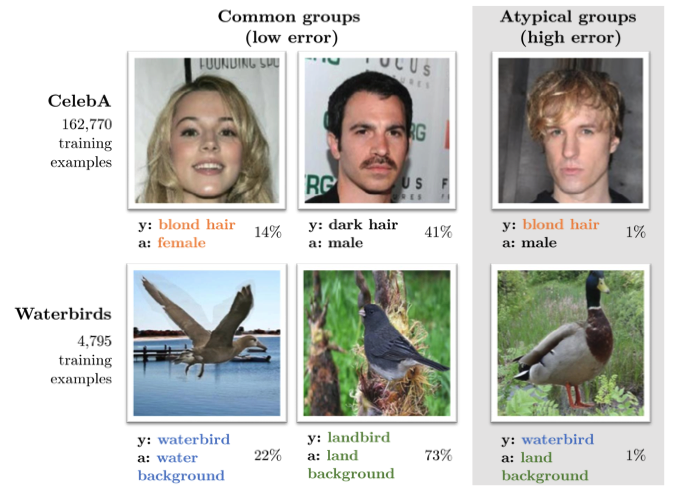
\includegraphics[scale=0.2]{sagawa_dataset.png}
    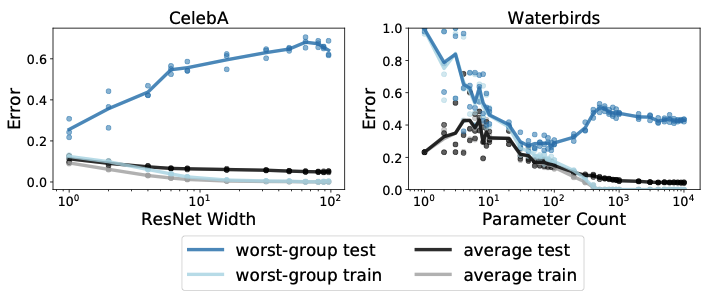
\includegraphics[scale=0.28]{sagawa_diagram_standard.png}
    \caption{Datasets used and results of a study on the effect of spurious correlations with varying model size conducted
    by Sagawa et al. \cite{pmlr-v119-sagawa20a}. It is clear to see that both ResNet and logistic regression have
    difficulty to classify atypical groups as their size increases despite having low training error on these groups.}
    \label{fig:sagawaImg}
\end{figure}

\subsection{How to mitigate the impact of spurious correlations between context and target}
\label{sec:contextSuppr}
Spurious correlations between context and target are among the most common spurious correlations and it is
therefore important to mitigate their impact on classification performance. The problem with such spurious correlations
is that they are not always harmful. The context that an object occurs with can also contain information which is helpful
for classification. So the challenge in such cases is to improve classification accuracy when an object occurs without
its context without compromising accuracy when an object co-occurs with its context. This was also the goal of a
new training procedure proposed by Singh et al. \cite{Singh_2020_CVPR} which works as follows
(overview in \hyperref[fig:contextSupprImg]{Figure 6}): \\
First, one needs to train a classifier on the given dataset which contains spurious correlations between labeled classes.
Note that the dataset needs to be multi-labeled. Next, for each class $c$ in the training set, a second class $d$ is
determined which co-occurs with $c$ frequently and which negatively impacts the prediction probability for class $c$ most.
To compute how class $d$ effects the prediction of class $c$ the following metric is used:  
\begin{align*}
    e_{sc}(c,d) = \frac{\frac{1}{|I_c \cap I_d|} \sum\limits_{i \in I_c \cap I_d}^{} p(i,c)}
    {\frac{1}{|I_c \textbackslash I_d|} \sum\limits_{i \in I_c \textbackslash I_d} p(i,c)}
\end{align*}
where $p(i,c)$ is the prediction probability for class $c$ being present in Image $i$ given by the classifier
trained in the beginning. A high $e_{sc}(c,d)$ indicates that the classifier relies on $d$ when predicting $c$
because the average prediction probability for $c$ drops significantly when $d$ is not present in the image. \\
According to metric $e_{sc}$, a list of the $K$ spurious correlations with the larget effect is compiled where $K$
is a parameter which can be chosen by the conductors of the algorithm beforehand. \\
Now during training, the goal of this training procedure is to train two disjoint feature subspaces for class $c$ and $d$
if the spurious correlation between $c$ and $d$ is in the compiled list. The idea is to split the weights which account
for class $c$ from those for class $d$. More precisely, if $x \in \mathbb{R}^N$ is the output of the final pooling layer
in the neural network trained on the dataset of interest the weights that $x$ is multiplied with can be denoted in a Matrix
$W \in \mathbb{R}^{N \times M}$ so that the output for the next layer is $y=W^Tx \in \mathbb{R}^M$. To obtain the two
feature subspaces, $W$ and $x$ are row-wise split randomly to obtain $W_c,W_d \in \mathbb{R}^{\frac{N}{2} \times M}$
and $x_c, x_d \in \mathbb{R}^{\frac{N}{2}}$. If class $c$ co-occurs with class $d$ during training, then $y$ is computed
as $y={W_c}^T x_c + {W_d}^T x_d$ meaning that the information gained from the co-occurring class is used for classification
and to adjust weights. So in this case, the training procedure is no different from that of a standard neural network.
However, if class $c$ occurs in absence of class $d$ then $y$ is computed as $y={W_c}^T x_c + {W_d}^T \bar{x}_d$ where
$\bar{x}_d$ is the average of $x_d$ over the last 10 mini-batches. In addition backpropagation on the weights of $W_d$
is disabled, meaning that only the weights belonging to $W_c$ are adjusted. Intuitively the neural network is forced to
learn from the information provided by class $c$ and the information obtained from the feature subspace of class $d$ is suppressed.
Note that $x_d$ could be set to any constant value. Setting $x_d = \bar{x}_d$ was a decision by Singh et al. which they state improves
stability during training. Also note that the neural network is only different from any standard neural network at training time. \\
The effectiveness of their algorithm was also shown in studies conducted by Singh et al. on the MS COCO dataset \cite{lin2015microsoft}:
they improved the accuracy for \enquote{ski} and \enquote{skateboard}, the two classes which were affected most by their context,
by 24.2 and 19.5 percentage points respectively. By inspecting the classifications made by a neural network trained with their
approach they verified that the network focuses on the object when is is present without its context while still letting the context contribute to the classification when it is present. \\
Overall, the approach proposed by Singh et al. is a promising one. Nevertheless, it fails to account for spurious correlations between
more than two classes. More problematic is that it only seems to effectively mitigate the impact of the most severe spurious correlations.
When investigating the 20 classes suffering from the most severe spurious correlations instead of the top 2, the performance increase
over a standard classifier shrinks to a mere 4.3 percentage points and the classification accuracy remains low at 28.8 \% when these
classes occur exclusively.

\begin{figure}
    \centering
    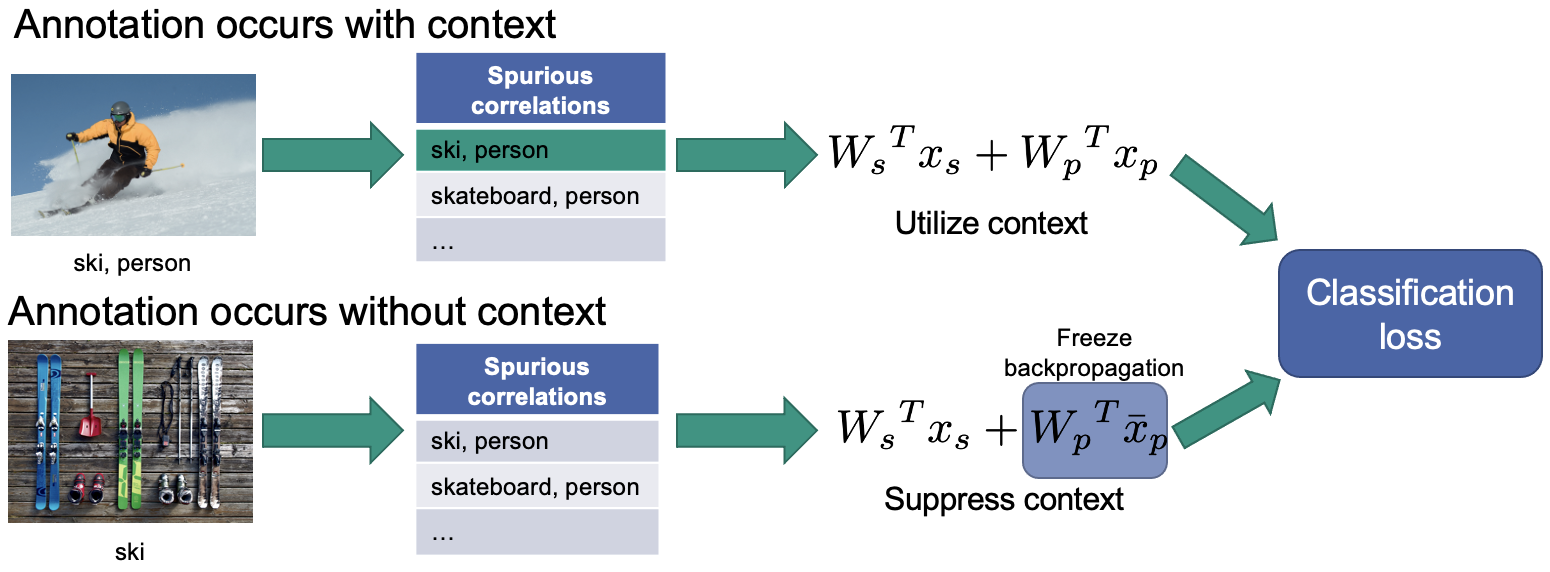
\includegraphics[scale=0.44]{context_suppression.png}
    \caption{Training procedure to reduce the effect of a spurious correlation between context and target, proposed
    by Singh et al. \cite{Singh_2020_CVPR}. If a label co-occurs with its spuriously correlated label, then training is
    no different from training any standard neural network. However, if a label occurs without its spuriously correlated
    label, then only the weights assigned to the dedicated label (ski in this example) are adjusted, forcing to the neural
    network to focus on the object in the image (ski).}
    \label{fig:contextSupprImg}
\end{figure}


\section{How to deal with datasets that might contain spurious correlations}
To summarize the findings of the previous sections, I have come up with a workflow on how to handle datasets that could contain spurious correlations.
An overview of the proposed workflow can be seen in \hyperref[fig:workflow]{Figure 7}. \\
The first step is to create or choose a dataset. Which of the two methods is the best depends largely on the target. If the goal is to classify or
detect common objects such as cars then it would be better to work with existing datasets such as CompCars in this case \cite{Yang_2015_CVPR}.
However, if the target is a rare or extraordinary concept such as a specific illness then the best approach is to create a dataset as most likely there will
not be any existing ones. In other cases, a hybrid approach could make sense. \\
After one has decided on which dataset to choose the next step is to scan the dataset for spurious correlations. In case time is not an issue
and volunteers are available the detection method of choice should be Crowdsourcing because it produces the best output, i.e. if finds the most spurious
correlations and estimates their degree best. If conducting Crowdsourcing is not feasible then I suggest a hybrid approach between Grad-CAM and TCAV which
combines the strengths of both algorithms: One should first train a neural network on the dataset chosen in step 1 and inspect its predictions with Grad-CAM
to come up with assumptions for spurious correlations. Next, one should check if these potential spurious correlations hold up with TCAV. \\
If the previous step did not lead to the detection of any spurious correlation, then the chosen dataset can be used for the given computer vision task. 
However, in the more likely scenario that one has found spurious correlations, the best way to go is to change or resample the dataset so that it no longer
contains the spurious correlations that were detected. After that one can start over with scanning the new dataset for spurious correlations again. \\
Unfortunately, obtaining new image data is not always possible, for example for legal or financial reasons. In that case, one has to adapt the neural network
to make it robust to the spurious correlations found in the dataset. Since the dataset could contain a spurious correlation between image angle and target
as well as a spurious correlation between context and target, one should focus on the prevailing spurious correlation which is the one with either
the highest weight (Crowdsourcing) or the highest TCAV-Score. \\
If the prevailing spurious correlation is between image angle and target, then using data augmentation (cropping, flipping and/or erasing parts of the image)
can be used to mitigate the impact of such a spurious correlation on classification accuracy. Research conducted by Agarwal et al. \cite{Agarwal_2020_CVPR}
supports this thesis. 
If the prevailing spurious correlation is between context and target, then I suggest using the context suppression algorithm presented in
\hyperref[sec:contextSuppr]{Section 4.2}. \\
Note that I have not mentioned any specific parameters to choose for the algorithms used in the workflow. Specific parameter choices depend on how restrictive
one wants to be when detecting spurious correlations. However it is important to note that most datasets of a certain size contain a least one spurious correlation.
Therefore the goal should not be to eliminate every single spurious correlation one has found by only the ones that lead to a significant loss in
classification accuracy. In addition, the suggested methods to mitigate the impact of a given spurious correlation are only simplified suggestions.
As mentioned before, mitigating the impact of spurious correlations has been studied to a greater extent than detecting them. To find out more about methods
to mitigate the impact of spurious correlations I refer to the sources mentioned in \hyperref[sec:mitigatingscs]{Section 4}.

%TODO: Bild ohne rote Unterstreichungen
\begin{figure}
    \centering
    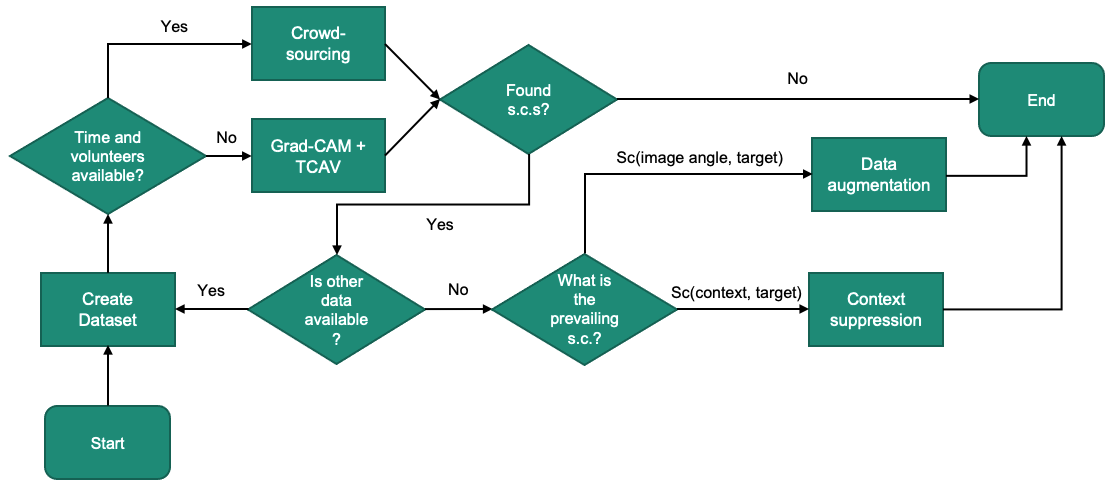
\includegraphics[scale=0.38]{sc_workflow.png}
    \caption{Workflow for dealing with image datasets that might contain spurious correlations}
    \label{fig:workflow}
\end{figure}


\section{Conclusion}
%TODO: Unexplored raus, Ende etwas netter formulieren
Overall, detecting spurious correlations in image datasets remains a challenging task mainly because feature extraction is difficult in image datasets and
because human intuition is needed in some part of the detection process to determine whether a correlation is spurious or not. \\
The existing approaches to detect spurious correlations have different strengths and weaknesses and should therefore be used under different circumstances: 
Crowdsourcing is the most effective approach but requires the most time and effort. TCAV and Grad-CAM can be conducted by only one person. 
Their strengths complement each other which makes it useful to combine both approaches. Nevertheless, all three methods have one significant downside: 
They require a large amount of human effort. Future research should therefore focus on automating the detection process, for example by automatically testing
a dataset for predefined concepts with TCAV (a similar approach has been proposed by Ghorbani et al. \cite{ghorbani2019automating}). \\
In general, mitigating the impact of spurious correlations on classification accuracy is well studied while detecting spurious correlations is
largely unexplored. It therefore seems like most researchers simply assume that their datasets contain a certain spurious correlation and see no need to
thoroughly examine their dataset to find out which spurious correlations it contains and how severe these are. However, properly checking a dataset for spurious
correlations is crucial in order to effectively mitigate their impact and further research is needed in this field due to the problems which the existing approaches
have to deal with.


\printbibliography

\end{document}